\section{Measurement with back-light illumination}
To measure the size and form of an object there are multiple ways. A popular way to get the contour is to place a light source behind the object desired to measure, and aim on the object with an camera. With this method the optical sensors get the silhouette of the object. 
\subsection{Light source}


\begin{figure}[ht]
	\centering
	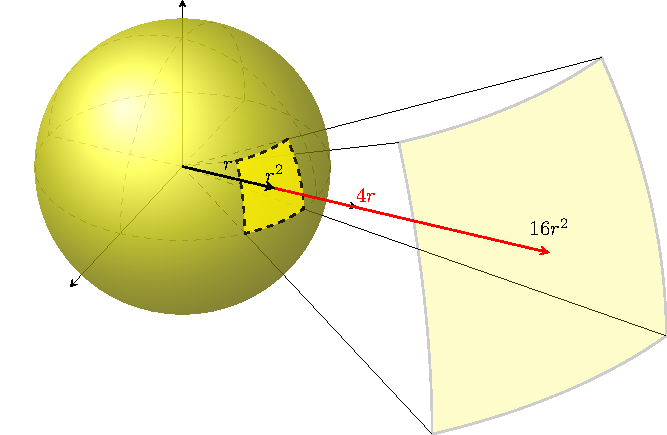
\includegraphics[width=0.9\textwidth]{2-theory/backlight/light.pdf}
	\caption{Light source in 3d\label{theory:light}}
\end{figure} 


\subsection{Light ray distribution}
\subsection{Light properties}
\subsection{Measurement precision changes}
\subsection{Image sensor properties}

